\documentclass{article}
\usepackage{enumerate}
\usepackage{amsmath}
\usepackage{amssymb}
\usepackage{graphicx}
\usepackage{subfigure}
\usepackage{geometry}
\usepackage{caption}
\usepackage{indentfirst}
\usepackage{tikz}
\usetikzlibrary{circuits.logic.US}
\usetikzlibrary{arrows.meta}
\usetikzlibrary{calc}
\geometry{left=3.0cm,right=3.0cm,top=3.0cm,bottom=3.0cm}
\renewcommand{\thesection}{Problem \arabic{section}.}
\title{VE270 Homework 4}
\author{Liu Yihao 515370910207}
\date{}

\newcommand{\drawmuxtwo}[3]{
	\draw #1 node (#2) [shape=rectangle,draw,minimum height=2cm,minimum width=2cm,text width=1cm,align=center] {#3};
	\draw (#2) ++(down:7.5mm) node {$s_0$};
	\draw (#2) ++(right:7.5mm) node {$d$};
	\draw (#2) ++(left:7.5mm) ++(up:2.5mm) node {$i_0$} ++(down:5mm) node {$i_1$};
}
\newcommand{\drawmuxfour}[3]{
	\draw #1 node (#2) [shape=rectangle,draw,minimum height=3cm,minimum width=2cm,text width=1cm,align=center] {#3};
	\draw (#2) ++(left:7.5mm) ++(up:7.5mm) node {$i_0$} ++(down:5mm) node {$i_1$} ++(down:5mm) node {$i_2$} ++(down:5mm) node {$i_3$};
	\draw (#2) ++(down:12.5mm)++(left:3.33mm) node {$s_1$} ++(right:6.66mm) node {$s_0$};
	\draw (#2) ++(right:7.5mm) node {$d$};
}
\newcommand{\drawmuxeight}[3]{
	\draw #1 node (#2) [shape=rectangle,draw,minimum height=5cm,minimum width=2cm,text width=1cm,align=center] {#3};
	\draw (#2) ++(left:7.5mm) ++(up:17.5mm) node {$i_0$} ++(down:5mm) node {$i_1$} ++(down:5mm) node {$i_2$} ++(down:5mm) node {$i_3$} ++(down:5mm) node {$i_4$} ++(down:5mm) node {$i_5$} ++(down:5mm) node {$i_6$} ++(down:5mm) node {$i_7$};
	\draw (#2) ++(down:22.5mm) node {$s_1$} ++(left:5mm) node {$s_2$} ++(right:10mm) node {$s_0$};
	\draw (#2) ++(right:7.5mm) node {$d$};
}
\newcommand{\drawdecodereight}[3]{
	\draw #1 node (#2) [shape=rectangle,draw,minimum height=5cm,minimum width=2cm,text width=1cm,align=center] {#3};
	\draw (#2) ++(right:7.5mm) ++(up:17.5mm) node {$d_0$} ++(down:5mm) node {$d_1$} ++(down:5mm) node {$d_2$} ++(down:5mm) node {$d_3$} ++(down:5mm) node {$d_4$} ++(down:5mm) node {$d_5$} ++(down:5mm) node {$d_6$} ++(down:5mm) node {$d_7$};
	\draw (#2) ++(left:7.5mm) node {$i_1$} ++(up:5mm) node {$i_0$} ++(down:10mm) node {$i_2$};
}
\newcommand{\drawfulladder}[3]{
	\draw #1 node (#2) [shape=rectangle,draw,minimum height=2cm,minimum width=2cm,text width=1cm,align=center] {#3};
	\draw (#2) ++(left:7.5mm) node {$c_o$};
	\draw (#2) ++(right:7.5mm) node {$c_i$};
	\draw (#2) ++(down:7.5mm) node {$s$};
	\draw (#2) ++(up:7.5mm) ++(left:3.3mm) node {$a$} ++(right:6.6mm) node {$b$};
}

\newcommand{\drawaddermodel}[3]{
	\draw #1 node (#2) [shape=rectangle,draw,minimum height=2cm,minimum width=4cm,text width=3cm,align=center] {#3};
	\draw (#2) ++(left:17.5mm) node {$c_o$};
	\draw (#2) ++(right:17.5mm) node {$c_i$};
	\draw (#2) ++(down:7.5mm) node {$s$};
	\draw (#2) ++(up:7.5mm) ++(left:10mm) node {$a$} ++(right:20mm) node {$b$};
}

\newcommand{\drawadder}[4]{
	\drawaddermodel{#1}{#2}{#3}
	\draw (#2) ++(up:10mm) ++(left:10mm) to node {$\diagup$} node[left] {8} ++(up:10mm) ;
	\draw (#2) ++(up:10mm) ++(right:10mm) to node {$\diagup$} node[left] {8} ++(up:10mm) ;
}

\newcommand{\drawsubtractor}[4]{
	\drawaddermodel{#1}{#2}{#3}
	\draw (#2) ++(up:10mm) ++(left:10mm) to node {$\diagup$} node[left] {8} ++(up:20mm);
	\draw (#2) ++(up:21.5mm) ++(right:10mm) node[not gate,point down] (#2__notgate) {#4 bit};
	\draw (#2) ++(up:10mm) ++(right:10mm) to node {$\diagup$} node[left] {#4} (#2__notgate.output);
	\draw (#2) ++(up:30mm) ++(right:10mm) to node {$\diagup$} node[left] {#4} (#2__notgate.input);
}


\begin{document}
\maketitle

\section{}
\begin{center}
\begin{tikzpicture}
\draw [help lines,dashed] (0,0) grid[xstep=2,ystep=3.5] (10,3.5);
\draw plot[const plot] coordinates {(0,2.5) (1,3) (2,2.5) (4,3) (5.5,2.5) (6,3) (7,2.5) (10,2.5)};
\draw plot[const plot] coordinates {(0,1.5) (2.5,2) (3.5,1.5) (8,2) (9,1.5) (10,1.5)};
\draw plot[const plot] coordinates {(0,1) (2.5,0.5) (4,1) (8,0.5) (10,0.5)};
\draw (-1,2.75) node {S} (-1,1.75) node {R} (-1,0.75) node {Q};
\end{tikzpicture}
\end{center}

\section{}
\begin{center}
\begin{tikzpicture}
\draw [help lines,dashed] (0,0) grid[xstep=2,ystep=3.5] (10,3.5);
\draw plot[const plot] coordinates {(0,3) (3.5,2.5) (4.5,3) (6.5,2.5) (9,3) (10,3)};
\draw plot[const plot] coordinates {(0,1.5) (1,2) (2,1.5) (3,2) (5.5,1.5) (7.5,2) (8.5,1.5) (10,1.5)};
\draw plot[const plot] coordinates {(0,0.5) (1,1) (3.5,0.5) (4.5,1) (7.5,0.5) (10,0.5)};
\draw (-1,2.75) node {D} (-1,1.75) node {G} (-1,0.75) node {Q};
\end{tikzpicture}
\end{center}

\section{}
\begin{center}
\begin{tikzpicture}
\draw [help lines,dashed] (0,0) grid[xstep=1.5,ystep=3.5] (11.5,3.5);
\draw plot[const plot] coordinates {(0,2.5) (1.5,3) (3,2.5) (4.5,3) (6,2.5) (7.5,3) (9,2.5) (10.5,3) (11.5,3)};
\draw plot[const plot] coordinates {(0,2) (0.75,1.5) (2.25,2) (3.75,1.5) (6.75,2) (8.25,1.5) (11.5,1.5)};
\draw plot[const plot] coordinates {(0,1) (1.5,0.5) (7.5,1) (10.5,0.5) (11.5,0.5)};
\draw (-1,2.75) node {Clock} (-1,1.75) node {D} (-1,0.75) node {Q};
\end{tikzpicture}
\end{center}

\section{}
\begin{center}
\begin{tikzpicture}
\draw [help lines,dashed] (0,0) grid[xstep=2,ystep=4.5] (11,4.5);
\draw plot[const plot] coordinates {(0,3.5) (1,4) (2,3.5) (3,4) (4,3.5) (5,4) (6,3.5) (7,4) (8,3.5) (9,4) (10,3.5) (11,3.5)};
\draw plot[const plot] coordinates {(0,2.5) (0.5,3) (3.25,2.5) (4.25,3) (5.25,2.5) (6.25,3)  (11,3)};
\draw plot[const plot] coordinates {(0,1.5) (0.75,2) (1.75,1.5) (5.25,2) (6.25,1.5) (7.25,2) (8.25,1.5) (11,1.5)};
\draw plot[const plot] coordinates {(0,0.5) (2,1) (6,0.5) (8,1) (11,1)};
\draw (-1,3.75) node {Clock} (-1,2.75) node {J} (-1,1.75) node {K} (-1,0.75) node {Q};
\end{tikzpicture}
\end{center}

\section{}
\begin{center}
\begin{tikzpicture}
\draw [help lines,dashed] (0,0) grid[xstep=2,ystep=4.5] (13,4.5);
\draw plot[const plot] coordinates {(0,3.5) (1,4) (2,3.5) (3,4) (4,3.5) (5,4) (6,3.5) (7,4) (8,3.5) (9,4) (10,3.5) (11,4) (12,3.5) (13,3.5)};
\draw plot[const plot] coordinates {(0,3) (3.5,2.5) (5.5,3) (9.5,2.5) (10.5,3) (13,3)};
\draw plot[const plot] coordinates {(0,2) (6.25,1.5) (8.5,2) (10.5,1.5) (13,1.5)};
\draw plot[const plot] coordinates {(0,1) (1,0.5) (3,1) (9,0.5) (9.5,1) (13,1)};
\draw (-1,3.75) node {Clock} (-1,2.75) node {PreN} (-1,1.75) node {T} (-1,0.75) node {Q};
\end{tikzpicture}
\end{center}

\section{}
\begin{center}
\begin{tikzpicture}[circuit logic US]
	\draw (0,-2.5) node [and gate,point left,scale=2] (g) {};
	\draw (g) -- ++(left:12cm);
	\foreach \i in {0,...,3} {
		\drawdflipflop{(-3.5*\i,0)}{f\i}{};
		\draw (f\i.east) ++(down:15mm) ++(right:5mm) node (Q\i) {$Q_\i$};
		\draw (Q\i) |- ($(f\i.east)+(down:2.5mm)$);
		\draw (f\i.west) ++(up:15mm) ++(left:5mm) node (i\i) {$i_\i$};
		\draw (i\i) |- ($(f\i.west)+(up:2.5mm)$);
		\draw (f\i.west) ++(down:2.5mm) -- ++(left:5mm) -- ++(down:22.5mm);
		\pgfgetlastxy{\x}{\y};
		\filldraw (\x,\y) circle [radius=0.5mm,fill];
	};
	\draw (g.input 1) ++(right:1cm) node (EN) {EN};
	\draw (g.input 2) ++(right:1cm) node (clock) {clk};
	\draw (g.input 1) -- (EN) (g.input 2) -- (clock);
\end{tikzpicture}
\end{center}

\section{}
\begin{center}
\begin{tikzpicture}[circuit logic US]
	\drawmuxfour{(4,4)}{m}{8-bit 4x1 mux};
	\draw (-4,9) node (C) {C};
	\draw (C) -- (-2.5,9) -- (-2.5,0);
	\foreach \i in {0,...,3} {
		\drawregister{(0,3*\i)}{r\i}{reg(8)}{8};
		\draw (r\i.west) -- ++(left:1.5cm);
		\ifnum \i>0
			\filldraw (r\i.south) ++(down:5mm) circle[radius=0.5mm];
			\filldraw (r\i.west) ++(left:1.5cm) circle[radius=0.5mm];
		\fi
	};
	\draw (r0.south) ++(down:5mm) -- ++(right:20mm) |- ($(m.west)+(down:7.5mm)$);
	\draw (r1.south) ++(down:5mm) -- ++(right:15mm) |- ($(m.west)+(down:2.5mm)$);
	\draw (r2.south) ++(down:5mm) -- ++(right:15mm) |- ($(m.west)+(up:2.5mm)$);
	\draw (r3.south) ++(down:5mm) -- ++(right:20mm) |- ($(m.west)+(up:7.5mm)$);
	\draw (m.south) ++(left:3.3mm) ++(down:1cm) node (s1) {$s_1$} ++(right:6.6mm) node (s0) {$s_0$};
	\draw (m.south) ++(left:3.3mm) -- (s1) (m.south) ++(right:3.3mm) -- (s0);
	\draw (m.east) ++(right:2cm) node (F) {F};
	\draw (m.east) to node {$\diagup$} node[above] {8} (F);
	\draw (r3.north) ++(up:1cm) node (D) {D};
	\draw (r3.north) -- (D);
	
\end{tikzpicture}
\end{center}

\section{}
\begin{center}
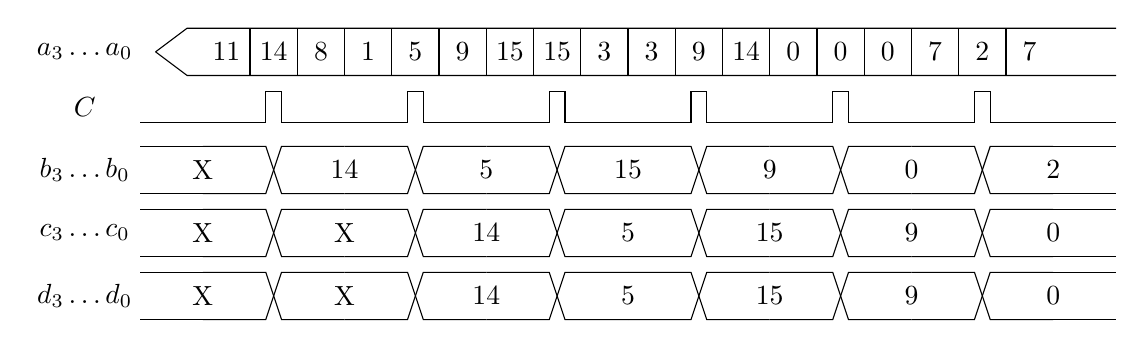
\begin{tikzpicture}[scale=0.8]
	\foreach \i/\val in {1/11,2/14,3/8,4/1,5/5,6/9,7/15,8/15,9/3,10/3,11/9,12/14,13/0,14/0,15/0,16/7,17/2,18/7} {
		\draw (\i*0.75,0) node {\val};
		\ifnum \i<18
			\draw (\i*0.75+0.375,0.375) -- ++(down:7.5mm);
		\fi
	};
	\draw (14.875,0.375) -- (0.125,0.375) -- (-0.375,0);
	\draw (14.875,-0.375) -- (0.125,-0.375) -- (-0.375,0);
	\foreach \i in {0,...,5} {
		\draw (3*0.75*\i+0.375,-1.5+0.375) -- ++(right:1cm) -- ++(up:5mm) -- ++(right:2.5mm) -- ++(down:5mm) -- ++(right:1cm);
	};
	\draw (0.375,-1.5+0.375) -- ++(left:1cm) (13.875,-1.5+0.375) -- ++(right:1cm);
	\foreach \j in {0,1,2} {
		\foreach \i in {0,...,5} {
			\draw (3*0.75*\i+0.375,-1.5-\j) -- ++(right:1cm) -- ++($(right:2.5mm)+(down:7.5mm)$) -- ++(right:1cm);
			\draw (3*0.75*\i+0.375,-2.25-\j) -- ++(right:1cm) -- ++($(right:2.5mm)+(up:7.5mm)$) -- ++(right:1cm);
		};
		\draw (0.375,-1.5-\j) -- ++(left:1cm) (13.875,-1.5-\j) -- ++(right:1cm);
		\draw (0.375,-2.25-\j) -- ++(left:1cm) (13.875,-2.25-\j) -- ++(right:1cm);
	};
	\foreach \i/\val in {0/X,1/14,2/5,3/15,4/9,5/0,6/2}
		\draw (3*0.75*\i+0.375,-1.875) node {\val};
	\foreach \i/\val in {0/X,1/X,2/14,3/5,4/15,5/9,6/0} {
		\draw (3*0.75*\i+0.375,-2.875) node {\val};
		\draw (3*0.75*\i+0.375,-3.875) node {\val};
	};
	\draw (-1.5,0) node {$a_3\dots a_0$};
	\draw (-1.5,-0.875) node {$C$};
	\draw (-1.5,-1.875) node {$b_3\dots b_0$};
	\draw (-1.5,-2.875) node {$c_3\dots c_0$};
	\draw (-1.5,-3.875) node {$d_3\dots d_0$};
\end{tikzpicture}
\end{center}




\end{document}
